%The PDF link
\documentclass[../structure.tex]{subfiles}
%\usepackage{../mypkg}
\begin{document}
\chapter{Method and Implementation}
As we implemented registration method, we are going to consider two objects, Target Graph $T$, which is remain fixed, and Template Graph $S$, which moves until it reach the optimal alignment with target graph $T$. To do so, we use Iterative Closest Point (ICP) as we mentioned before, for each point on template graph $S$ we look for closest point on target graph $S$. Then we start moving each point in $S$ to correspondent point in $T$ with respect to stiffness.

\section{Data preparation}
In this thesis we follow the method in \cite{Amberg2007} which implemented for surface graphs. Due to difference between the data used in \cite{Amberg2007} which is surface graphs saved in points cloud format or mesh format, and our data which is pathways in streamlines format saved in \textit{ply} file as shown in figure [\ref{fig:data}]. Thus we had to build a tool for reading \textit{ply} file format as streamlines and build graphs out of it, each \textit{ply} file has one pathway.

Then we build a cost function which we will discuss next. 

\begin{figure}[h!]
\centering
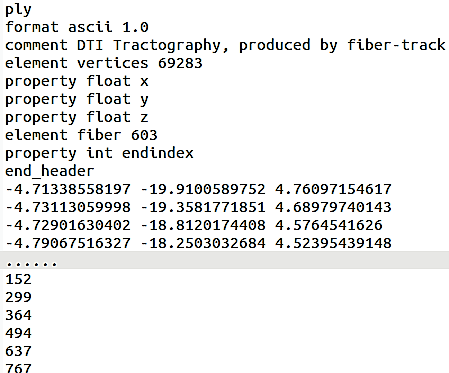
\includegraphics[scale=0.5]{002_data}
\captionsetup{justification=centering}
\caption{A sample of a Brain pathway saved in a \textit{ply} file.}
\label{fig:data}
\end{figure}

\subsection{The PLY file}
Let us illustrate a bit the \textit{ply} file we use to save our data as shown in figure [\ref{fig:data}]. It consist of two parts, header and body. The header consist of all information that necessary to pars the file, and the body has the data itself.
\begin{itemize}
\item The first line represent the file type.
\item The second line is the file format.
\item The third line is comment.
\item The forth line is first group of elements (as \textit{ply} can have many) name and number (each element in one line). It shows that we have 69283 vertices.
\item The 5th, 6th and 7th lines shows that the first group of elements has three properties, each of them in float format and the name of each property.
\item The 8th line shows the second group of elements which has 603 fiber tract and so on.
\item The 10th line shows the end of the header part.
\item The remaining lines is the body of the file which has all the data, each element in one line.
\end{itemize}

\section{Cost Function}
The simplest form of our cost function is shown in the equation (\ref{equ:equation1}):

\begin{equation}
\label{equ:equation1}
||Ax-b||^2
\end{equation}

This simple format of the cost function makes it easy to solve by \textit{Least Square (LSQR)} algorithm which implemented in \textit{scipy.sparse.linalg.lsqr}, but to be practical and implement this cost function we need to divide it to three terms as shown in equation (\ref{equ:costFun}), distance term, stiffness term, and landmark term.

\begin{equation}
E(X) = E_{d}(X) + \alpha E_{s}(X) + \beta E_{t}(X)
\label{equ:costFun}
\end{equation}

\subsection{Distance Term}
The first part of the cost function is distance term as shown in (\ref{equ:costFun}), it represent the accumulation of distance between each point in template graph and the target graph 
 to understand it better lets put it in a new equation ():

\end{document}